\section{Modelo de Datos}

La base de datos está implementada en \textbf{PostgreSQL 15} administrado por Supabase. El diseño cumple con la \textbf{Tercera Forma Normal (3FN)} y sigue las siguientes convenciones:

\begin{itemize}
    \item Nombres de tablas en singular.
    \item Nombres de columnas en \texttt{snake\_case}.
    \item Clave primaria: \texttt{id} (UUID generado con \texttt{gen\_random\_uuid()}).
    \item Claves foráneas: \texttt{tabla\_id} (ej: \texttt{student\_id}, \texttt{level\_id}).
    \item Columnas de fecha/hora: \texttt{TIMESTAMPTZ}.
\end{itemize}

\section{Diagrama Entidad-Relación}

\begin{figure}[H]
\centering
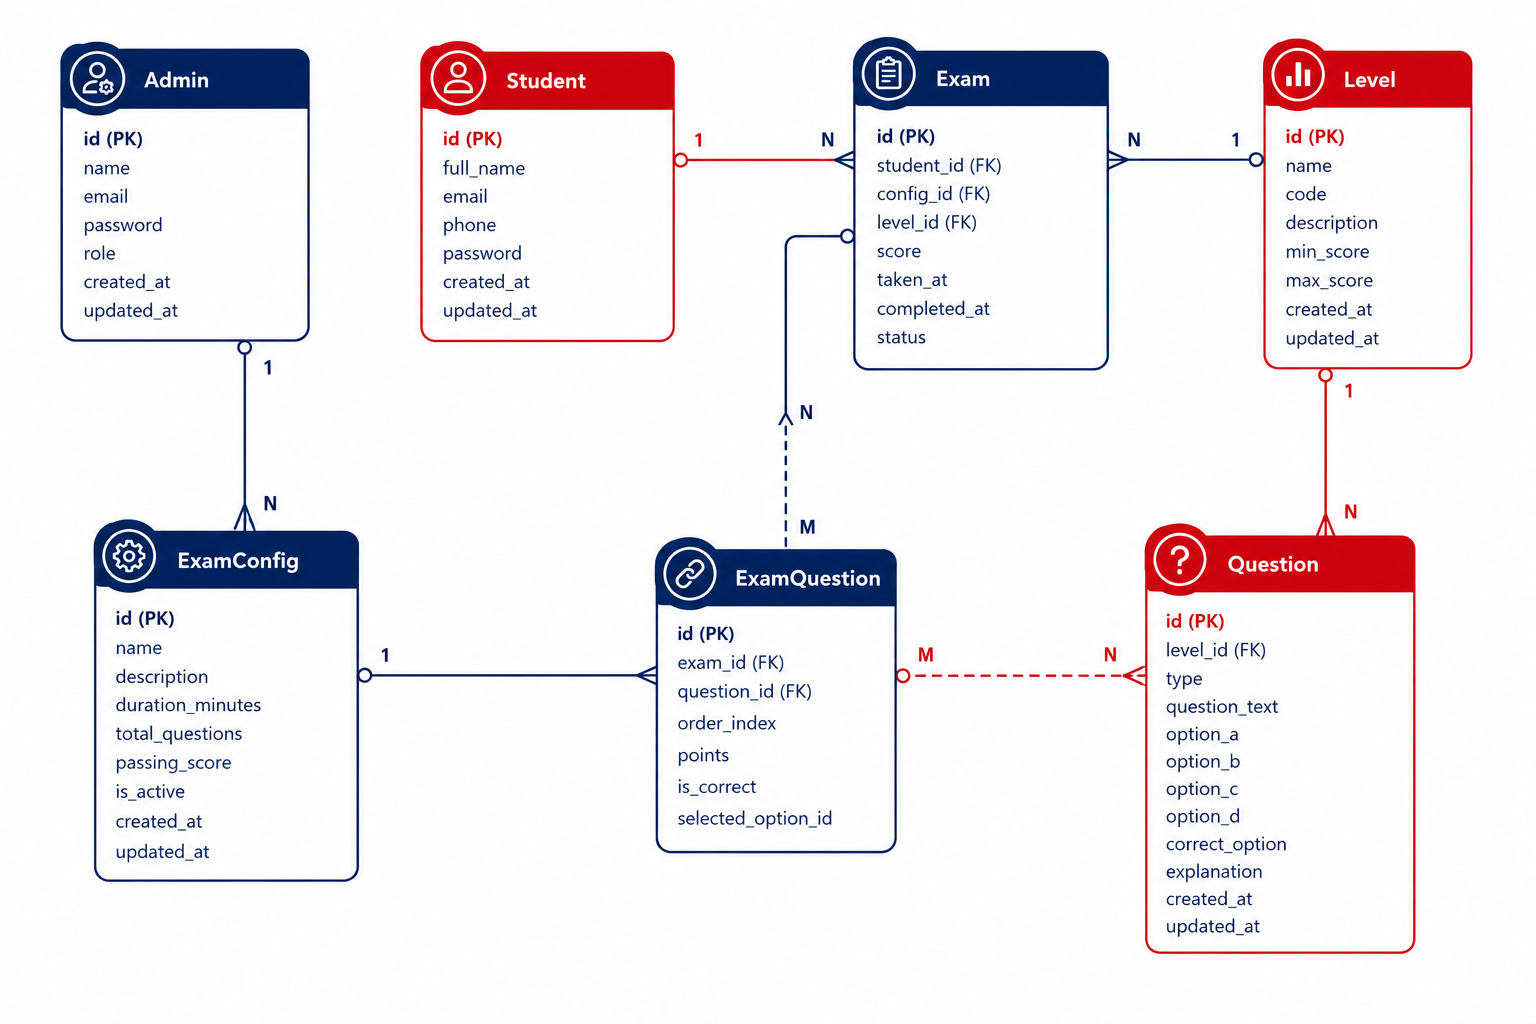
\includegraphics[width=\textwidth]{imagenes/diagrama-conceptual.png}
\caption{Diagrama Entidad-Relación (modelo conceptual)}
\end{figure}

\begin{figure}[H]
\centering
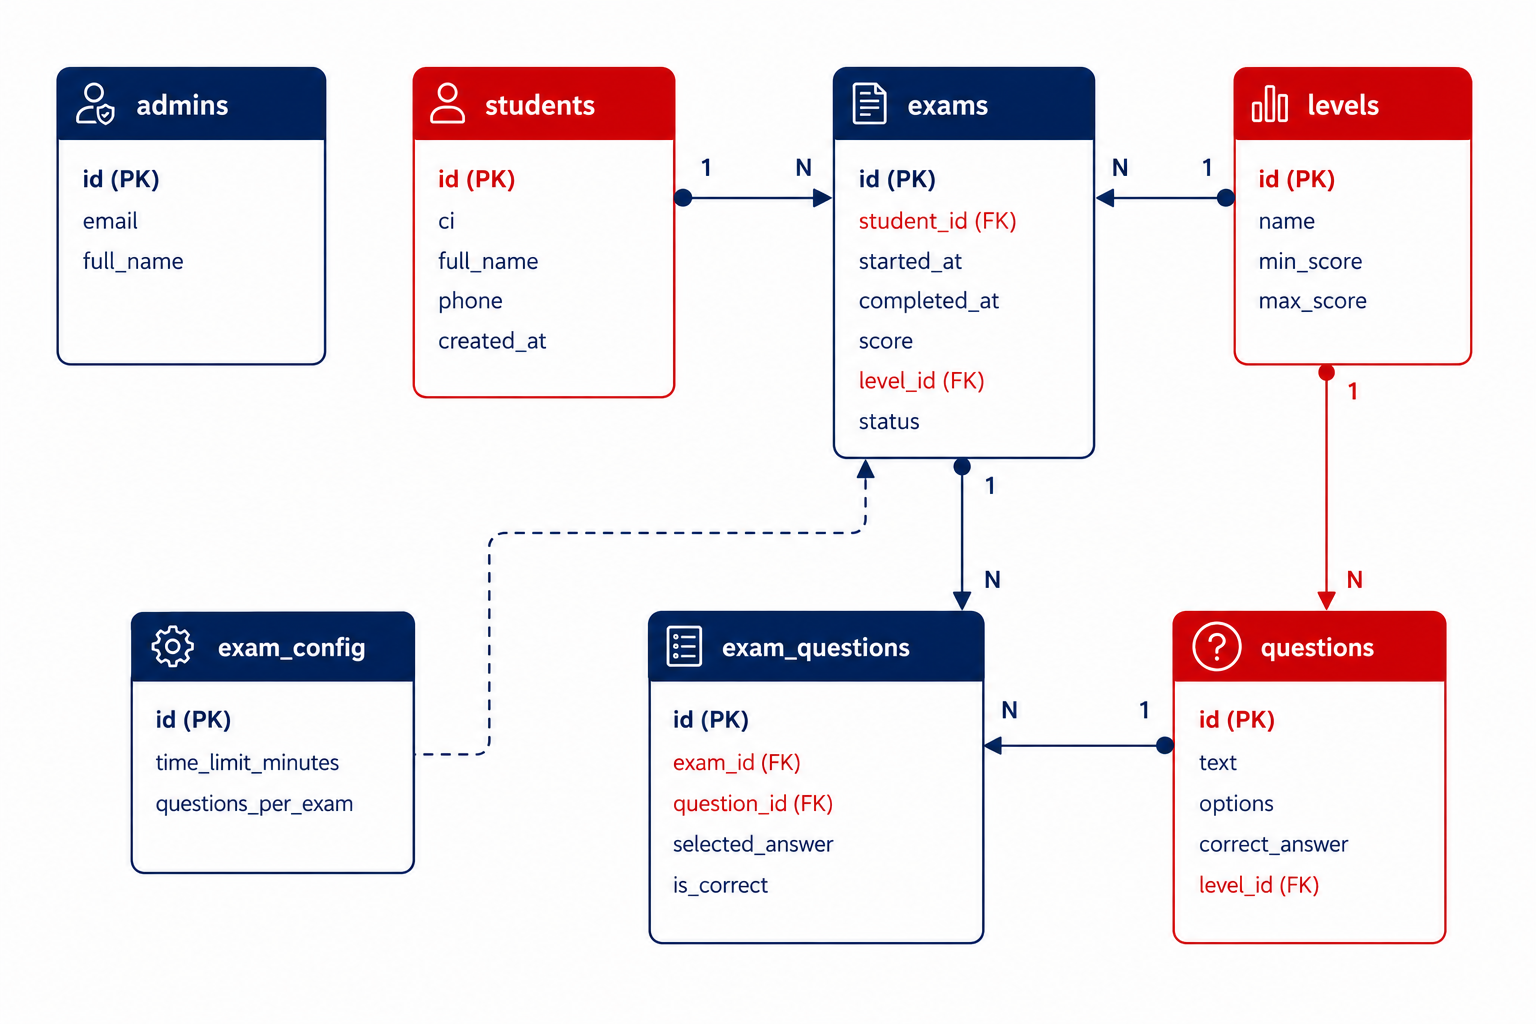
\includegraphics[width=\textwidth]{imagenes/diagrama-relacional.png}
\caption{Diagrama Relacional (tablas con columnas)}
\end{figure}

\section{Diagrama UML Definitivo}

A partir del diseño conceptual y relacional, se consolidó el esquema final de la base de datos con 10 tablas interconectadas. A continuación se presentan dos versiones del diagrama completo:

\begin{figure}[H]
\centering
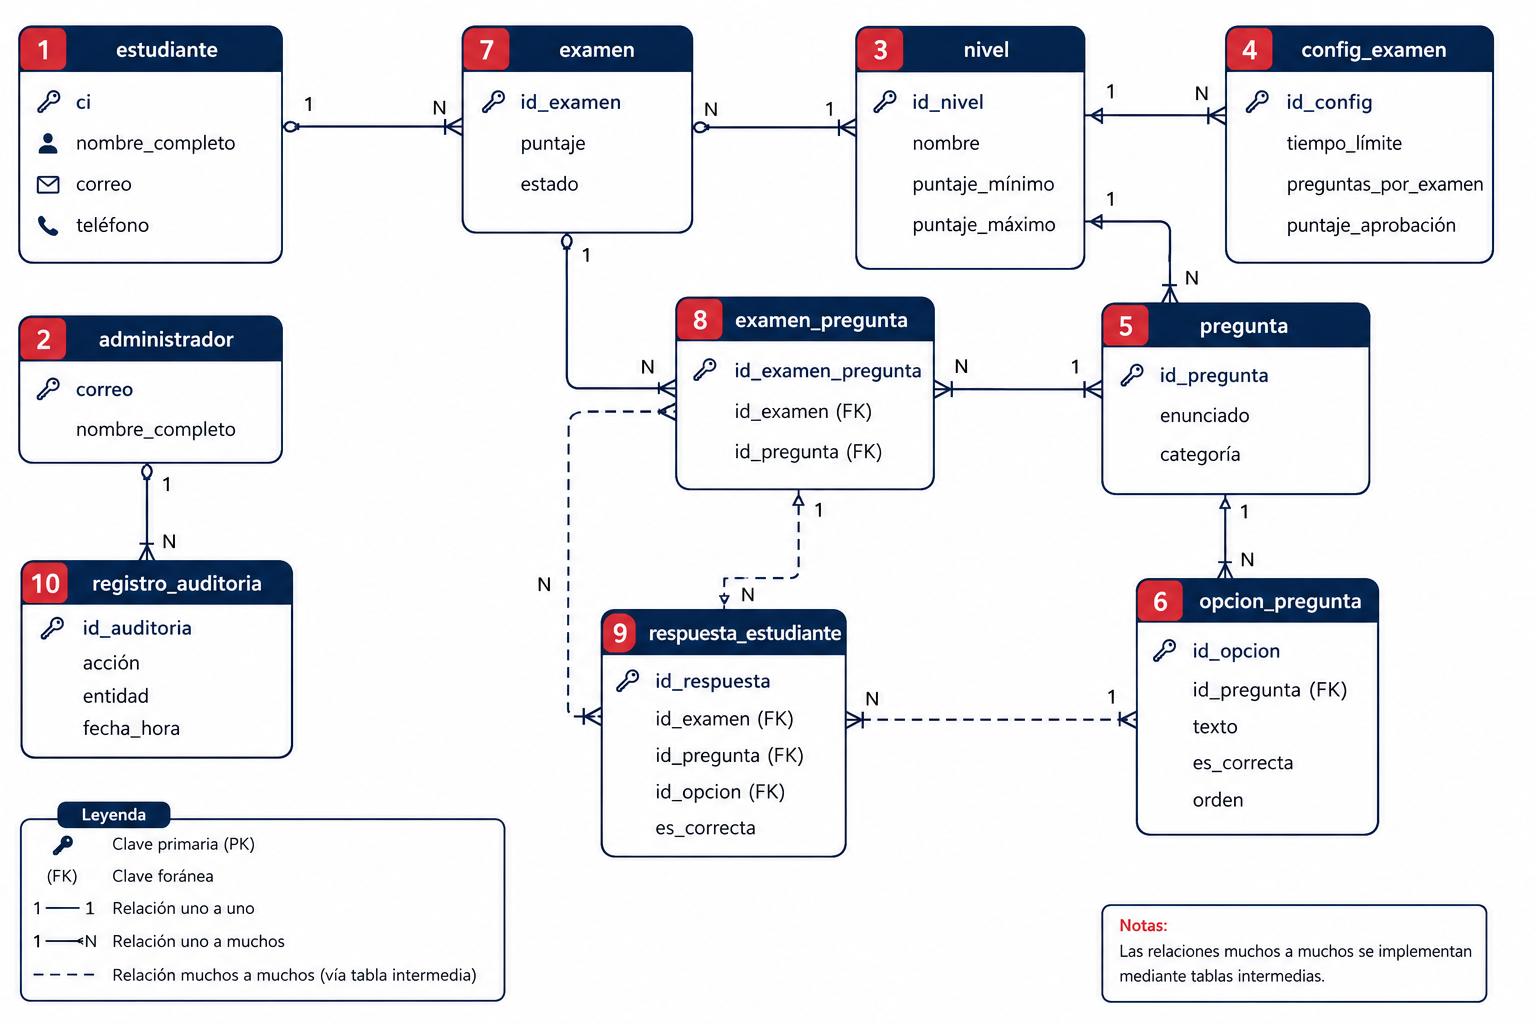
\includegraphics[width=\textwidth]{imagenes/Imagen-10-Tablas.png}
\caption{Diagrama visual de las 10 tablas (vista estética)}
\end{figure}

\begin{figure}[H]
\centering
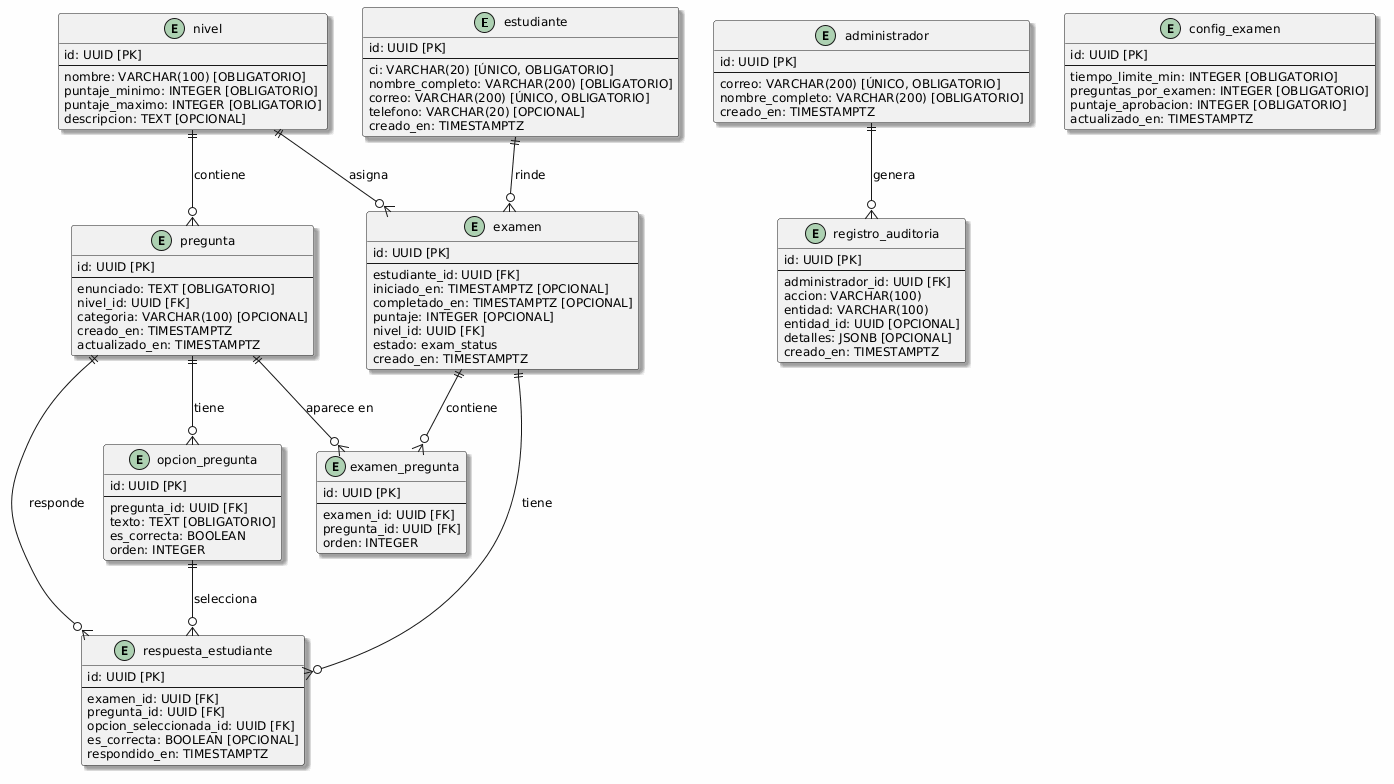
\includegraphics[width=\textwidth]{imagenes/Diagrama-UML-10-Tablas.png}
\caption{Diagrama UML preciso con columnas, tipos y relaciones (generado con PlantUML)}
\end{figure}

\section{Tablas}

\subsection{student}

Almacena los datos de los estudiantes registrados en el sistema.

\begin{longtable}{l l l p{5cm}}
\toprule
\textbf{Columna} & \textbf{Tipo} & \textbf{Restricción} & \textbf{Descripción} \\
\midrule
\endhead
id & UUID & PK & Identificador único \\
ci & VARCHAR(20) & NOT NULL, UNIQUE & Carnet de Identidad (login) \\
full\_name & VARCHAR(200) & NOT NULL & Nombre completo \\
email & VARCHAR(200) & NOT NULL, UNIQUE & Correo electrónico (login alterno) \\
phone & VARCHAR(20) & NULLABLE & Teléfono de contacto \\
created\_at & TIMESTAMPTZ & NOT NULL & Fecha de registro \\
\bottomrule
\caption{Tabla \texttt{student}}
\end{longtable}

\subsection{admin}

Almacena los datos de los administradores del sistema.

\begin{longtable}{l l l p{5cm}}
\toprule
\textbf{Columna} & \textbf{Tipo} & \textbf{Restricción} & \textbf{Descripción} \\
\midrule
\endhead
id & UUID & PK & Identificador único \\
email & VARCHAR(200) & NOT NULL, UNIQUE & Correo electrónico (login) \\
full\_name & VARCHAR(200) & NOT NULL & Nombre completo \\
created\_at & TIMESTAMPTZ & NOT NULL & Fecha de registro \\
\bottomrule
\caption{Tabla \texttt{admin}}
\end{longtable}

\subsection{level}

Define los niveles de inglés con sus rangos de puntaje, basados en el Marco Común Europeo de Referencia para las Lenguas (MCERL).

\begin{longtable}{l l l p{5cm}}
\toprule
\textbf{Columna} & \textbf{Tipo} & \textbf{Restricción} & \textbf{Descripción} \\
\midrule
\endhead
id & UUID & PK & Identificador único \\
name & VARCHAR(100) & NOT NULL & Nombre del nivel \\
min\_score & INTEGER & NOT NULL, CHECK($\ge$ 0) & Puntaje mínimo \\
max\_score & INTEGER & NOT NULL & Puntaje máximo \\
description & TEXT & NULLABLE & Descripción del nivel \\
\bottomrule
\caption{Tabla \texttt{level}}
\end{longtable}

\newpage

\subsection{question}

Banco de preguntas del sistema, cada una asociada a un nivel específico.

\begin{longtable}{l l l p{5cm}}
\toprule
\textbf{Columna} & \textbf{Tipo} & \textbf{Restricción} & \textbf{Descripción} \\
\midrule
\endhead
id & UUID & PK & Identificador único \\
text & TEXT & NOT NULL & Enunciado de la pregunta \\
level\_id & UUID & FK $\rightarrow$ level.id, NOT NULL & Nivel al que pertenece \\
category & VARCHAR(100) & NULLABLE & Categoría (grammar, vocabulary, reading) \\
created\_at & TIMESTAMPTZ & NOT NULL & Fecha de creación \\
updated\_at & TIMESTAMPTZ & NOT NULL & Fecha de modificación \\
\bottomrule
\caption{Tabla \texttt{question}}
\end{longtable}

\subsection{question\_option}

Opciones de respuesta para cada pregunta. Se normalizan en una tabla separada en lugar de usar arrays JSON.

\begin{longtable}{l l l p{5cm}}
\toprule
\textbf{Columna} & \textbf{Tipo} & \textbf{Restricción} & \textbf{Descripción} \\
\midrule
\endhead
id & UUID & PK & Identificador único \\
question\_id & UUID & FK $\rightarrow$ question.id, NOT NULL & Pregunta asociada \\
text & TEXT & NOT NULL & Texto de la opción \\
is\_correct & BOOLEAN & NOT NULL, DEFAULT FALSE & Indica si es la respuesta correcta \\
order & INTEGER & NOT NULL, CHECK($\ge$ 0) & Orden de la opción \\
\bottomrule
\caption{Tabla \texttt{question\_option}}
\end{longtable}

\textbf{Restricciones adicionales:} UNIQUE(question\_id, order) evita opciones duplicadas en una pregunta. Cada pregunta debe tener exactamente una opción correcta.

\subsection{exam\_config}

Configuración global del examen. Funciona como \textit{singleton} — una sola fila activa define los parámetros del sistema.

\begin{longtable}{l l l p{5cm}}
\toprule
\textbf{Columna} & \textbf{Tipo} & \textbf{Restricción} & \textbf{Descripción} \\
\midrule
\endhead
id & UUID & PK & Identificador único \\
time\_limit\_minutes & INTEGER & NOT NULL, CHECK($>$ 0) & Tiempo límite en minutos \\
questions\_per\_exam & INTEGER & NOT NULL, CHECK($>$ 0) & Cantidad de preguntas por examen \\
passing\_score & INTEGER & NOT NULL, CHECK(0-100) & Puntaje mínimo de aprobación (\%) \\
updated\_at & TIMESTAMPTZ & NOT NULL & Fecha de modificación \\
\bottomrule
\caption{Tabla \texttt{exam\_config}}
\end{longtable}

\newpage

\subsection{exam}

Registro de cada examen rendido por un estudiante.

\begin{longtable}{l l l p{5cm}}
\toprule
\textbf{Columna} & \textbf{Tipo} & \textbf{Restricción} & \textbf{Descripción} \\
\midrule
\endhead
id & UUID & PK & Identificador único \\
student\_id & UUID & FK $\rightarrow$ student.id, NOT NULL & Estudiante que rinde el examen \\
started\_at & TIMESTAMPTZ & NULLABLE & Fecha de inicio \\
completed\_at & TIMESTAMPTZ & NULLABLE & Fecha de finalización \\
score & INTEGER & NULLABLE, CHECK($\ge$ 0) & Puntaje obtenido (\%) \\
level\_id & UUID & FK $\rightarrow$ level.id, NULLABLE & Nivel asignado \\
status & exam\_status & NOT NULL, DEFAULT 'pending' & Estado del examen \\
created\_at & TIMESTAMPTZ & NOT NULL & Fecha de creación \\
\bottomrule
\caption{Tabla \texttt{exam}}
\end{longtable}

\textbf{exam\_status (ENUM):} \texttt{pending} | \texttt{in\_progress} | \texttt{completed}

\subsection{exam\_question}

Relación muchos-a-muchos entre examen y preguntas. Define qué preguntas específicas tuvo cada examen y en qué orden.

\begin{longtable}{l l l p{5cm}}
\toprule
\textbf{Columna} & \textbf{Tipo} & \textbf{Restricción} & \textbf{Descripción} \\
\midrule
\endhead
id & UUID & PK & Identificador único \\
exam\_id & UUID & FK $\rightarrow$ exam.id, NOT NULL & Examen asociado \\
question\_id & UUID & FK $\rightarrow$ question.id, NOT NULL & Pregunta asociada \\
order & INTEGER & NOT NULL, CHECK($\ge$ 0) & Orden de la pregunta \\
\bottomrule
\caption{Tabla \texttt{exam\_question}}
\end{longtable}

\textbf{Restricción adicional:} UNIQUE(exam\_id, question\_id) evita preguntas duplicadas.

\subsection{student\_answer}

Respuesta individual a cada pregunta dentro de un examen.

\begin{longtable}{l l l p{5cm}}
\toprule
\textbf{Columna} & \textbf{Tipo} & \textbf{Restricción} & \textbf{Descripción} \\
\midrule
\endhead
id & UUID & PK & Identificador único \\
exam\_id & UUID & FK $\rightarrow$ exam.id, NOT NULL & Examen asociado \\
question\_id & UUID & FK $\rightarrow$ question.id, NOT NULL & Pregunta asociada \\
selected\_option\_id & UUID & FK $\rightarrow$ question\_option.id & Opción seleccionada \\
is\_correct & BOOLEAN & NULLABLE & Indica si es correcta \\
answered\_at & TIMESTAMPTZ & DEFAULT NOW() & Fecha de respuesta \\
\bottomrule
\caption{Tabla \texttt{student\_answer}}
\end{longtable}

\newpage

\subsection{audit\_log}

Registro de auditoría para todas las acciones administrativas.

\begin{longtable}{l l l p{5cm}}
\toprule
\textbf{Columna} & \textbf{Tipo} & \textbf{Restricción} & \textbf{Descripción} \\
\midrule
\endhead
id & UUID & PK & Identificador único \\
admin\_id & UUID & FK $\rightarrow$ admin.id, NULLABLE & Administrador que realizó la acción \\
action & VARCHAR(100) & NOT NULL & Tipo de acción (CREATE, UPDATE, DELETE) \\
entity & VARCHAR(100) & NOT NULL & Tabla afectada \\
entity\_id & UUID & NULLABLE & ID del registro afectado \\
details & JSONB & NULLABLE & Detalles adicionales \\
created\_at & TIMESTAMPTZ & NOT NULL & Fecha de la acción \\
\bottomrule
\caption{Tabla \texttt{audit\_log}}
\end{longtable}

\section{Funciones SQL}

\subsection{Cálculo de Nivel}

Determina el nivel de inglés correspondiente a un puntaje obtenido:

\begin{lstlisting}[language=PostgreSQL, caption=Función \texttt{fn\_calculate\_level}]
CREATE OR REPLACE FUNCTION fn_calculate_level(p_score INTEGER)
RETURNS UUID AS $$
DECLARE
    v_level_id UUID;
BEGIN
    SELECT id INTO v_level_id
    FROM level
    WHERE p_score BETWEEN min_score AND max_score
    ORDER BY min_score ASC
    LIMIT 1;

    RETURN v_level_id;
END;
$$ LANGUAGE plpgsql STABLE;
\end{lstlisting}

\subsection{Selección Aleatoria de Preguntas}

Selecciona preguntas al azar del banco para conformar un examen:

\begin{lstlisting}[language=PostgreSQL, caption=Función \texttt{fn\_get\_random\_questions}]
CREATE OR REPLACE FUNCTION fn_get_random_questions(p_count INTEGER)
RETURNS TABLE (id UUID) AS $$
BEGIN
    RETURN QUERY
    SELECT q.id
    FROM question q
    ORDER BY RANDOM()
    LIMIT p_count;
END;
$$ LANGUAGE plpgsql STABLE;
\end{lstlisting}

\subsection{Finalización de Examen}

Calcula el puntaje final, asigna el nivel y actualiza el registro del examen:

\begin{lstlisting}[language=PostgreSQL, caption=Función \texttt{fn\_complete\_exam}]
CREATE OR REPLACE FUNCTION fn_complete_exam(p_exam_id UUID)
RETURNS TABLE (score INTEGER, level_id UUID, level_name VARCHAR) AS $$
DECLARE
    v_score     INTEGER;
    v_level_id  UUID;
    v_level_name VARCHAR;
    v_total     INTEGER;
    v_correct   INTEGER;
BEGIN
    -- Contar respuestas correctas
    SELECT COUNT(*) INTO v_correct
    FROM student_answer sa
    WHERE sa.exam_id = p_exam_id AND sa.is_correct = TRUE;

    SELECT COUNT(*) INTO v_total
    FROM student_answer sa
    WHERE sa.exam_id = p_exam_id;

    -- Calcular porcentaje
    v_score := ROUND((v_correct::NUMERIC / v_total) * 100);

    -- Obtener nivel
    SELECT l.id, l.name INTO v_level_id, v_level_name
    FROM level l
    WHERE v_score BETWEEN l.min_score AND l.max_score
    ORDER BY l.min_score ASC
    LIMIT 1;

    -- Actualizar examen
    UPDATE exam
    SET score = v_score,
        level_id = v_level_id,
        completed_at = NOW(),
        status = 'completed'
    WHERE id = p_exam_id;

    RETURN QUERY SELECT v_score, v_level_id, v_level_name;
END;
$$ LANGUAGE plpgsql;
\end{lstlisting}

\section{Triggers}

\begin{itemize}
    \item \textbf{trg\_check\_daily\_exam}: Impide que un estudiante rinda más de un examen por día. Se ejecuta antes de INSERT en la tabla \texttt{exam}.
    \item \textbf{trg\_prevent\_historical\_change}: Impide modificar respuestas de un examen que ya fue completado. Se ejecuta antes de UPDATE en \texttt{student\_answer}.
    \item \textbf{trg\_question\_updated\_at}: Actualiza automáticamente la columna \texttt{updated\_at} en \texttt{question}.
\end{itemize}
